\documentclass[11pt]{article}

\usepackage[]{ACL2023}

\usepackage{times}
\usepackage{latexsym}

\usepackage[T1]{fontenc}

\usepackage[utf8]{inputenc}

\usepackage{microtype}

\usepackage{inconsolata}

\usepackage{graphicx}

\title{Asking Clarifying Questions for Conversational Search}

\author{
  Ansh Bisht \and
  Jordan Dickson \and
  Jack Harrison \and
  Ruben Lazell \and
  Andrew Taison  \\
  School of Computing, Engineering and the Built Environment, \\
  Edinburgh Napier University \\
  Matric Numbers: 40527530, 40545300, 40537035, 40679914, 40538519
}


\begin{document}
\maketitle
\begin{abstract}
Short abstract.
\end{abstract}


\section{Introduction}
Brief context of problem - why clarifying Q's matter.
What is the goal.
Structure of the paper.

\section{Related Work}
Existing systems, prior research etc.

\section{Methodology}



\subsection{System Overview}
The system for the clarification model was constructed through a series of key components:User queries with a question for the system, RASA for application control of the entire system, Best Matching 25 (BM25) model for matching the queries on the Wikipedia Dataset, and SBERT for constructing Sentence Similarity Scores to rank the most appropriate question.

\newline

The dependencies and relationships of these components are illustrated Figure 1.

\begin{figure}[htbp]
  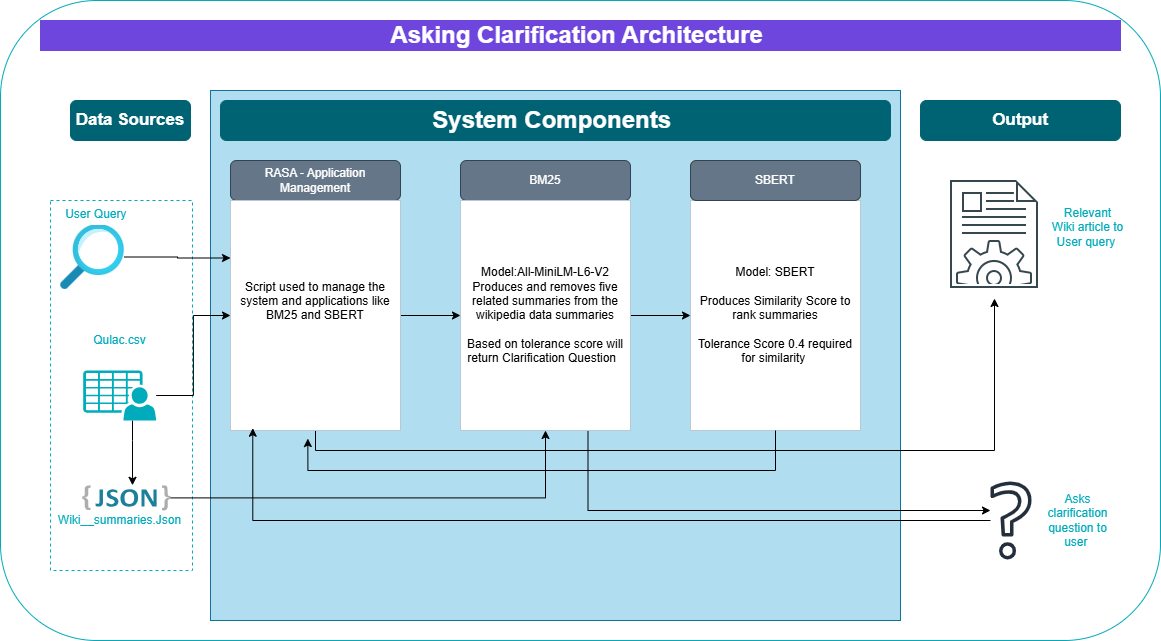
\includegraphics[width=\linewidth]{./img/system_diagram.png}
  \caption{System Diagram for our Clarification project}
  \label{fig:sys_diag}
\end{figure}

\subsection{Qulac Dataset}
The Qulac - short for Questions for Lack of Clarity—is a benchmark dataset created to support research on asking clarifying questions in open-domain, information-seeking conversations and was one of the primary datasets for this system. One of the initial steps was to appropriately shape the data to work with the other elements within our system. The transformations for cleaning this dataset were performed initially in Python using the Pandas library, and the resulting CSV was stored within GitHub.

\subsection{Original Qulac Dataset}
In short the Qulac dataset is a dictionary with query keys and a list of relevant facet descriptions (user intents).

Each query in Qulac is paired with a set of ten candidate clarifying questions, which are designed to resolve potential ambiguity. For example, the query "jaguar" could relate to the animal, the car brand, or even the sports team, and Qulac includes questions such as “Are you referring to the animal or the car brand?” to help systems distinguish between these interpretations. These questions were manually authored and assessed through crowdsourcing to ensure relevance and effectiveness in eliciting more specific user intent. Queries are also accompanied by retrieved web passages from the ClueWeb09 Category B corpus, providing context for question evaluation.

The dataset includes annotations from human judges who rated each candidate question based on its helpfulness, relevance, and clarity. The ratings fall into categories such as excellent, good, fair, or bad, offering a rich signal for training supervised learning models. These annotations allow for the creation of ranking systems that prioritize better clarifying questions over less helpful ones. The inclusion of such human judgments positions Qulac as a valuable dataset for evaluating both neural ranking models and question generation systems in the conversational IR domain.

\subsection{Clean Qulac Schema}
\renewcommand{\arraystretch}{1.2} % increase row height for readability

\begin{table}[ht]
  \centering
  \caption{Transformed Qualac Dataset for BM25 and Wiki Summaries}
  \label{tab:dataset-columns}
  \begin{tabular}{@{} l l p{5cm} @{}}
    \hline
    \textbf{Column Name}  & \textbf{Type}    & \textbf{Description}                        \\ 
    \hline
    Index                 & String           & Facet index based on word string.            \\ 
    Category Name         & String           & Name of the broader category of the dataset. \\ 
    Facet Description     & String           & Detailed description of the facet.           \\ 
    Col 1                 & String           & Response 1.                                  \\ 
    Col 2                 & String           & Response 2.                                  \\ 
    Col 3                 & String           & Response 3.                                  \\ 
    Col 4                 & String           & Response 4.                                  \\ 
    New Index             & Integer          & Row index counter.                           \\ 
    \hline
  \end{tabular}
\end{table}

One of the most important features of the Qulac Dataset was the facet descriptions, as they were used to derive the Wikipedia Summaries. A facet is a clarifying intent subtopic to given a query and an facet description is a description of this subtopic. Let us take "Cat" as an example of a facet. In this scenario there are four potential facets for cats; the mammal - felius catus - , the musical  and the shoe brand. The facet description are important as they context to  derive from a readable form which of these facets are being used in a certain context. Hence they important for deriving the correct wikipedia summaries. 

\subsection{Wikipedia Summaries}
The Wikipedia summaries were generated using a series of GET responses contained within a Python script on the Wikipedia API. The aim was to generate five summaries per topic based on the facet descriptions \textendash{} relating to the user's query. In short, the facet descriptions were used within a search function as to return the most relevant results within a given context. The reason why five results where generated instead of all possible results was reduce the amount of noise in our dataset. Only the Wikipedia summaries where used to save on performance and time. In a larger and more extensive project, the entire Wikipedia summary should be generated. 

\begin{figure}[htbp]
  \centering
  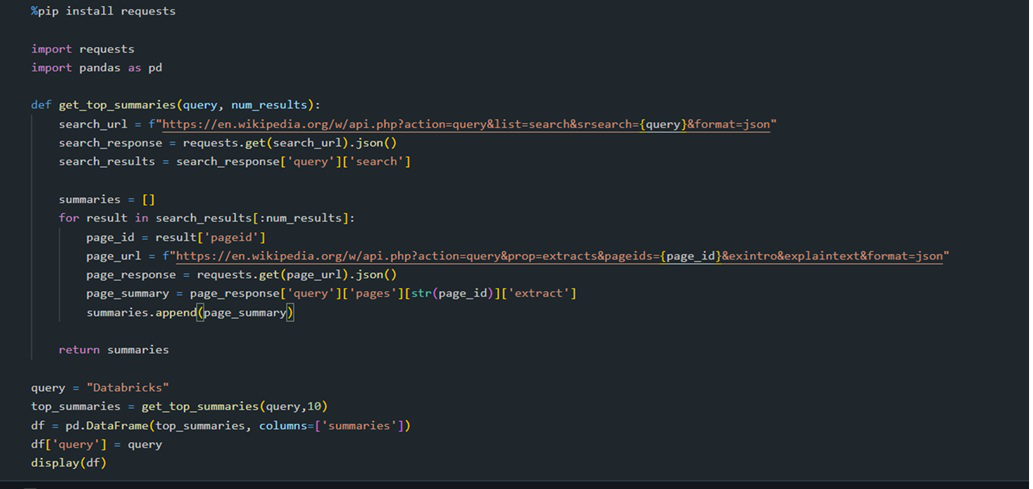
\includegraphics[width=\linewidth]{./img/wiki.png}
  \caption{Wikipedia Summaries Generation}
  \label{fig:wikipedia method}
\end{figure}

In the figure - wikipedia method, a function is used to generate the results of our searches. The method was crafted in this way to ensure that it could retrieve data from the API at ease. If the project was larger in scope, the parameters and a couple of variables could be simply changed to gain the entire wikipedia article. 

Once completed, the Wikipedia Summaries were shaped into the cleaned dataset above. These summaries were required for BM25 later in the project. In a larger project, the Wikipedia API could be used to return the entire articles, but this would come at a cost of time, compute, and complexity.


\subsection{{RASA}}
RASA is the machine learning framework used for building this system. It is used to manage the dialogue by deploying the suitable modules. For this project, RASA deploys BM25 and SBERT, allowing the system to function cohesively. 

\subsection{Best Matching 25 (BM25)}
BM25 was a key ranking function used in the project for informational retrieval within the project. For the project, BM25 ranked the user queries to the relevant Wikipedia summaries giving them a ranking score. This function was imported from Huggingface via a python script. 
 \newline
 \newline
The documents used were the Wikipedia Summaries from the generated CSV. A ranking was also performed using all-MiniLM-L6-v2 from HuggingFace to select the best matching summary.


\subsection{SBERT}
The final step was determining the suitability of the top-ranked question. A specialized version of BERT called SBERT from Huggingface was utilised.

Our SBERT model was fine-tuned on \texttt{sbert\_training\_data.csv}, which contained two features: context and question. Each context is a formatted string combining the initial query and the next element. The model would try to find a similarity between the two strings to rank the relevant results.





\section{Evaluation}
How did we check the system works.
Describe testing process.

\section{Results and Discussion}
Sample outputs.
Summary of system behaviour.
What worked well, what didn't?
Possible improvements.

\section{Conclusion}
start here.

\section*{Limitations}
Required by ACL format, and should be AFTER conclusion.
Discuss honest limitations of the work.

\section*{Ethics Statement}
Required by ACL format. Could just be a sentence or two.
Explicit ethics statement on the broader impact of the work, or other ethical considerations.

\bibliographystyle{acl_natbib}
\bibliography{references}

\appendix

\section{Appendix}
Possibly not needed.

\end{document}
